\documentclass[15pt]{ctexart}
\usepackage{xeCJK}
	\setCJKmainfont{SimSun}         % 缺省中文字体为宋体
	\setmainfont{Times New Roman}   % 缺省英文字体 Times New Roman
\usepackage{geometry}
	% \geometry{left=2.5cm,right=2.5cm,top=2.5cm,bottom=3.5cm}
	\geometry{bottom=3.5cm}
\usepackage{float}
\usepackage{listings}
\usepackage{graphicx}
\usepackage{appendix}
\usepackage[colorlinks]{hyperref}
\usepackage{amsmath}
\usepackage{indentfirst}
\usepackage{enumerate}
\usepackage{fancyhdr}
\usepackage{textcomp}
\usepackage{appendix} 
\usepackage{multirow}
\usepackage{geometry}
\geometry{verbose,letterpaper}
\usepackage{media9}
\pagestyle{fancy}
\lhead{应用层——C/S与P2P通信}
\rhead{\thepage}
\cfoot{}
\lstset{frameshape={RYRYNYYYY}{yny}{yny}{RYRYNYYYY}, backgroundcolor=\color[RGB]{245,245,244}}

\begin{document}
\begin{titlepage}
    \centering
    
\includegraphics[width=1\textwidth]{imgs/SYSULogo.png}\par\vspace{1cm}
    \vspace{1cm}
    {\scshape\huge 应用层通信 \\ 项目报告 \\ \centering \scshape \Huge C/S与P2P通信 \par}
    \vspace{1.5cm}
    {\Large\bfseries \flushleft 学院:数据科学与计算机学院 \\ 专业:计算机科学与技术 \\ 年级:2016级 \\组长(学号):王锡淮(16337236)\\组员(学号):杨陈泽(16337271)\\
    组员(学号):肖遥(16337258)\par}
    % \vspace{2cm}

% Bottom of the page
    % {\large \today\par}
\end{titlepage}
\tableofcontents
\newpage
\section{项目介绍} % (fold)
\label{sec:项目介绍}
\par 这是一个应用层的通信应用项目,包括一个服务器-客户端模型和P2P模型,两者的功能都是传输文件,项目主页是\url{https://github.com/Leo-xh/C-S-and-P2P-demo}。其中,服务器-客户端模型使用的是单服务器多客户端模型,并且单一客户端可以同时请求多个文件,服务器和客户端都使用多线程模型。P2P模型参考的是bittorrent协议,完成了bittorrent协议的一个实现(命名为Compact Bittorrent Protocol/1.0),并且实现了原来的biitorrent协议中的几个扩展协议。
	\subsection{设计应用层协议的原则} % (fold)
	\label{sub:设计应用层协议的原则}
		一个应用层协议应当包含两个主要部分:
		\begin{enumerate}
			\item 编码控制(编码和译码)。
			\item 流程控制。
		\end{enumerate}
		\par 一个协议可以根据多种原则来进行划分,比如按照编码分类、按照协议边界分类。而对于协议的评判来讲,主要有四点评判原则:
		\begin{enumerate}
			\item 协议的高效性,包括打包和解包的效率、数据压缩率等等。关于这一点,应用层协议的效率主要涉及数据方面,因为数据的传输并不是应用层的责任。
			\item 协议的简单性。
			\item 协议的可扩展性。举个例子,在Bittorrent协议中,有许多扩展,本项目中也实现了几个扩展,这些扩展使得Bittorrent更加健壮和高效。
			\item 协议应当向前和向后兼容。拿上面的Bittorrent扩展为例,实现了这些扩展的协议版本兼容了为实现这些扩展的协议版本。
		\end{enumerate}
		\par 设计协议时,主要需要回答三个基本问题:
		\begin{enumerate}
			\item 这个协议需要完成什么问题。
			\item 协议中传输的信息的含义是什么。
			\item 该协议的特征是什么。
		\end{enumerate}
		下面本项目中设计的协议都将围绕这三个问题。
	% subsection 设计应用层协议的原则 (end)
% section 项目介绍 (end)
\section{C/S通信} % (fold)
\label{sec:c_s通信}
\par 本项目中实现的C/S通信模型使用python实现,主要利用的是socket,threading,struct,os等常用库,其中服务器使用多线程,能够支持多个客户端同时请求文件;客户端也使用多线程,能够同时请求多个文件。
\par 提供的服务如下:
\begin{enumerate}[1.]
	\item 原始数据传输。
	\item 加密数据传输。
	\item 查看服务器的文件目录。
\end{enumerate}
\subsection{协议设计} % (fold)
\label{sub:协议设计}
\par 这是一个二进制模糊边界和固定边界的协议,即传输的数据以二进制编码,在请求报文中能够确定报文长度,在应答报文中无法明确知道协议报文的长度,需要通过报文中的长度字段知道。
\par 在设计协议格式时,经过小组的讨论,决定在协议头中采用两种(请求和发文件)报文格式,请求报文头中有:类型、服务、版本、序号和文件名字段,而发文件报文头中有:类型、服务、版本、序号、长度、错误码和数据体;
每个字段的作用在后面有相应解释。定义好协议格式后,接着定义客户端和服务器之间的行为交互:首先客户端在链接上服务器时,1、可以向服务器发出“查询文件目录”请求,
然后服务器查询本地的文件及目录,以明文形式发回去给客户端,客户端拿到后输出回显到屏幕上;2、客户端发出“某文件”请求,并选择是否需要加密,服务器接收请求,若文件不存在,发送一个错误码为1的报文
给客户端,客户端根据该报文做出响应;若文件存在,服务器将文件分成许多报文向客户端发送(根据加密需要选择加密与否),并且服务器在自己的终端上显示发送文件时的进度条,
等文件的所有报文发送完成,服务器再向客户端发送一个数据长度为0的报文,告知客户端,文件发送完毕。
\par 接着分析了该应用层协议是用来传输二进制文件(主要功能)和传输明文(次要功能),对于明文来说,就不得不考虑编码转换的问题,
因为需要采用了struct库的pack和unpack函数来进行压包和解包的。而且,在明确了该应用层协议是采用TCP之后,我们进行了下面的TCP缺陷分析:
\par 在实现这个通信模型时会遇到的问题主要是TCP协议的分包和粘包问题,TCP中只有数据流这样的概念,而没有数据包这一类的概念;
因为自己设计应用层调用网络编程的API接口,一次调用中要发送的报文大小在API接口中没有规定,但是在机器的IP层,TCP并不是按照
调用者传给API的报文大小一次性发出(我们已经知道在以太网中TCP报文大小限制在1500bytes),而是采用自己的算法,将包切割,
然后发出,包到达对方的IP层时再进行重组(TCP提供了可靠的服务,不需要考虑丢包问题),但是由于IP层的算法设计,导致接收方的IP层
重组后的传给应用层的报文,并不一定完全等于发送方的应用层传给IP层的报文,会可能出现:分包(发送方应用层的一个报文,实际上分成了两个接收方应用层的报文)
和粘包(发送方应用层一个报文的部分(或者全部)与另一个报文的部分(或者全部),实际上合成接收方应用层的一个报文)。
每次收到的不一定会是一个完整的数据包,所以需要通过某种方法明确当前处理的数据包的大小,然后解析这个大小的数据包。
\par 这类问题的解决方法大致有两种:第一种是,设计一个独特的分隔符,将应用层的每个包后面加上该分隔符,然后接收方根据分隔符来
分割出每个包,但是因为我们这次传输的是文件(二进制),无法预测可以采用什么充当分隔符而不会在文件上出现;第二种是:发送方在报文协议头上,
加上一个字段,表明该报文数据字段的长度,然后接收方的应用层设置一个报文缓冲区,每个到达的报文存在缓冲区中,
首先在缓冲区中提取报文头(固定长度的),然后根据报文头的长度字段再在缓冲区中提取相应长度的数据字段(当缓冲区现有数据长度小于需要提取的长度时,继续收包,
直到长度大于等于需要提取的长度),这样便能完全解决由于TCP数据流的特点而产生的缺陷问题。我们本次协议采用的是第二种方案。
\par 至于在加密过程中,我们采用的是AES对称加密算法,原因是:对称加密,适合数据的加密和加密;而且实现较为简单。

\par 客户端的请求报文设计如表\ref{tab:client}所示。
\begin{table}[H]
	\centering
	\begin{tabular}{|c|c|c|c|}
		\hline
		类型 & 服务 & 版本 & 序号 \\
		\hline
		\multicolumn{4}{|c|}{\multirow{6}*{文件名}
		}
		\\
		\multicolumn{4}{|c|}{~}\\
		\multicolumn{4}{|c|}{~}\\
		\multicolumn{4}{|c|}{~}\\
		\multicolumn{4}{|c|}{~}\\
		\multicolumn{4}{|c|}{~}\\
		\multicolumn{4}{|c|}{~}\\
		\multicolumn{4}{|c|}{~}\\
		\hline
	\end{tabular}
	\caption{客户端请求报文}
	\label{tab:client}
\end{table}
\par 参数解释如下:类型指的是协议号,服务是服务号(3种不同的服务),版本是协议版本号,序号是请求序号,大小都是2字节,文件名指的是请求的文件名,长度上限为200字节。
\par 服务器响应报文设计如表\ref{tab:server}:
\begin{table}[H]
	\centering
	\begin{tabular}{|c|c|c|c|c|c|}
		\hline
		类型 & 服务 & 版本 & 序号 & 长度 & 错误码 \\
		\hline
		\multicolumn{6}{|c|}{\multirow{6}*{数据}}
		\\
		\multicolumn{6}{|c|}{~}\\
		\multicolumn{6}{|c|}{~}\\
		\multicolumn{6}{|c|}{~}\\
		\multicolumn{6}{|c|}{~}\\
		\multicolumn{6}{|c|}{~}\\
		\multicolumn{6}{|c|}{~}\\
		\multicolumn{6}{|c|}{~}\\
		\hline
	\end{tabular}
	\caption{服务器应答报文}
	\label{tab:server}
\end{table}
\par 类型、服务、版本、序号字段和请求报文中一样,长度字段指的是数据字段的长度,大小为2字节,数据字段是发送往客户端的数据。
\par 对于上面提到的三种服务,对应的服务号分别是0,1,2。
\par 而错误码字段现在只有两种:0表示服务器有客户端需要的文件;1表示服务器没有客户端需要的文件。
\par 服务器和客户端的控制流程如图\ref{fig:server}和\ref{fig:client}所示。
\begin{figure}[H]
	\begin{minipage}{0.5\linewidth}
		\flushleft
		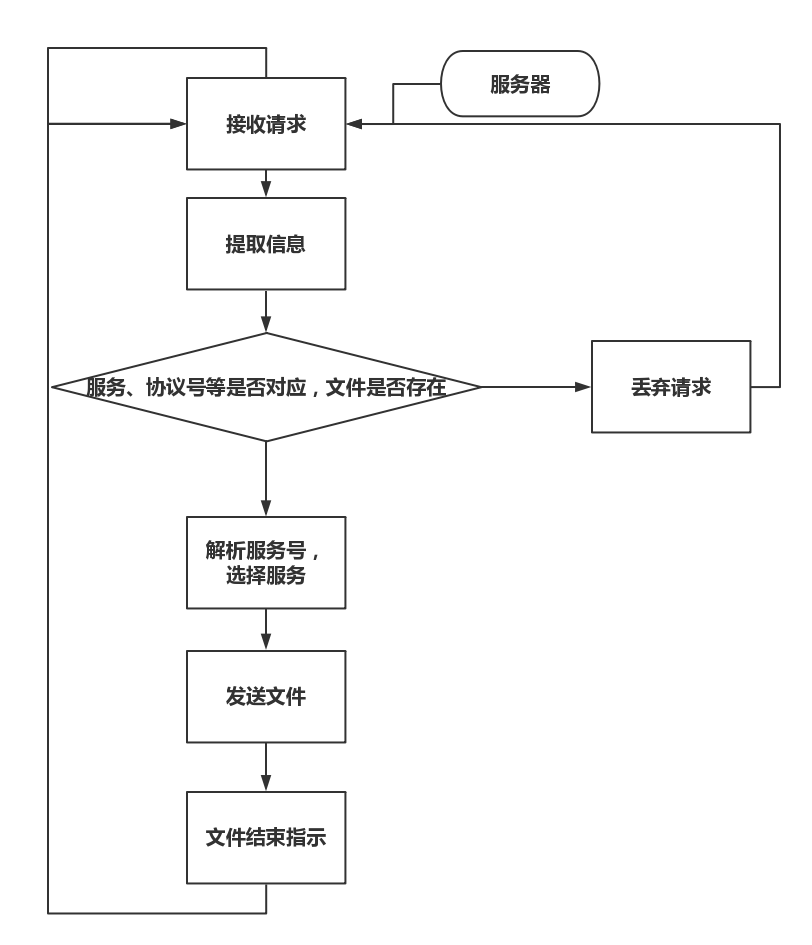
\includegraphics[width=1.1\linewidth]{imgs/server.png}
		\caption{服务器流程图}
		\label{fig:server}
	\end{minipage}
	\begin{minipage}{0.45\linewidth}
		\flushright
		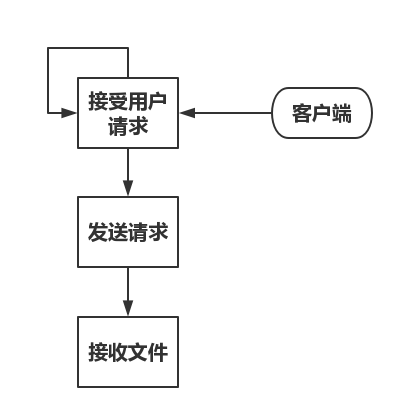
\includegraphics[width=1\linewidth]{imgs/client.png}
		\caption{客户端流程图}
		\label{fig:client}
	\end{minipage}
\end{figure}
% subsection 协议设计 (end)
\subsection{特点} % (fold)
\label{sub:特点}
本项目中实现的C/S模型的特点是:
\begin{enumerate}
	\item 实现了支持多文件同时传输文件时的传输进度条,即多个进度条能够同时正常显示。
	\item 实现了服务器的文件查找功能。
	\item 使用了数据加密技术。
	\item 客户端能够同时请求多个文件,服务器能够同时处理多个请求。
\end{enumerate}
% subsection 特点 (end)

% section c_s通信 (end)

\section{P2P通信} % (fold)
\label{sec:p2p通信}
	本项目中完成了bittorrent协议的一个实现(命名为Compact Bittorrent Protocol/1.0),这个实现采用了基本的Bittorrent协议规定的内容,同时参考了社区中的建议(比如Block大小的选择)。同时我们参考了Bittorrent协议网站上列出的的扩展方案中的协议。我们的实现主要包括两个方面,一是客户端(Peer在和Tracker通信时作为客户端)与服务器(Tracker)的通信;二是对等方之间的通信。下面将围绕这两个方面进行介绍。
	\subsection{Tracker和Client的通信} % (fold)
	\label{sub:tracker_和_client}

		\subsubsection{协议设计} % (fold)
		\label{ssub:协议设计}
		
		% subsubsection 协议设计 (end)
		\subsubsection{协议特点} % (fold)
		\label{ssub:协议特点}
		
		% subsubsection 协议特点 (end)
	% subsection tracker_和_client (end)
	\subsection{Peer通信} % (fold)
	\label{sub:peer通信}
	
		\subsubsection{协议设计} % (fold)
		\label{ssub:协议设计}
			
		% subsubsection 协议设计 (end)
		\subsubsection{协议特点} % (fold)
		\label{ssub:协议特点}
			
		% subsubsection 协议特点 (end)
	
	% subsection peer通信 (end)

% section p2p通信 (end)

\section{安装和部署} % (fold)
\label{sec:安装和部署}

% section 安装和部署 (end)

\section{结果} % (fold)
\label{sec:结果}
\subsection{结果展示} % (fold)
\label{sub:结果展示}
\par """"插入结果展示""""
\\
\\
\\
\\
\\
\\
\\
\\
\\
\\
\\
% subsection 结果展示 (end)
\subsection{对比} % (fold)
\label{sub:对比}

% subsection 对比 (end)

% section 结果 (end)
\section{总结} % (fold)
\label{sec:总结}

% section 总结 (end)

\section{项目管理记录} % (fold)
\label{sec:项目管理记录}

% section 项目管理记录 (end)

\newpage
\appendixpage
\begin{appendices}
	\section{参考文献} % (fold)
	\begin{enumerate}
		\item Jonas Fonseca,et al,\url{http://jonas.nitro.dk/bittorrent/bittorrent-rfc.html#anchor17},Bittorrent协议详细解读。
		\item Bram Cohen,\url{http://www.bittorrent.org/beps/bep_0003.html},Bittorrent官方协议。
	\end{enumerate}
	% section  (end)
\end{appendices}

\end{document}